\begin{frame}{Data Processing}
    \begin{block}{}
        Data for the traditional assets were downloaded from Bloomberg while the cryptocurrency data was retrieved from CoinMetrics. This was then cleaned so that all assets had data points on all the given dates.
    \end{block}   
    \begin{block}{}
       We then calculated the daily returns of the assets which allowed us to conduct the exploratory data analysis.
    \end{block} 
    \begin{block}{}
        For comparability reasons, the futures were rolled on a monthly basis. All price time series start on 30/09/2015 and end on 18/11/2022. For the main part of the following analysis, a time period
beginning in 2020 was used.
    \end{block} 
 \begin{alertblock}{}
    An Asset class is an effective hedging tool if its returns are negatively correlated to those of crypto currencies.
    \end{alertblock} 
\end{frame}

\begin{frame}{Correlation}
    \begin{block}{}
     We created a heatmap of the correlations between the assets. This allowed us to construct our hedging portfolios.
    \end{block} 
    
\begin{figure}
        \centering
    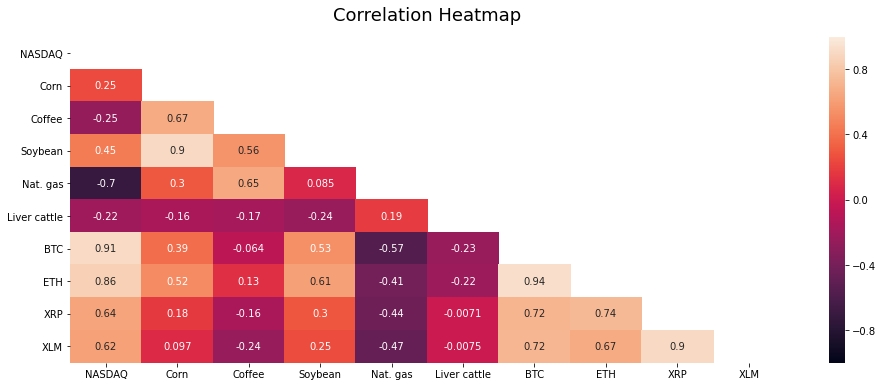
\includegraphics[scale=0.35]{images/illustrate/heatmap_small.png}
        \caption{Correlations between asset classes.}
\end{figure}
\end{frame}

\begin{frame}{Hedging Portfolios}
    \begin{block}{}
     Each portfolio contained an equally weighted investment part (the cryptocurrency) and a hedging part.
    \end{block}   
    \begin{alertblock}{}
The generalised construction of the daily return of such a portfolio on day $t$ is given by:
\begin{equation} \label{eq:pfform}
\mu_t^{PF} = \frac{1}{2} \cdot \left( \frac{\sum_{i=1}^K{\mu_{t}^{i}}}{K} + \mu_{t}^{Hedge} \right)
\end{equation}
Where $\mu$ is the time series of returns of a given portfolio consisting of $K+1$ components. 
    \end{alertblock} 
    \begin{block}{}
The following performance metrics were then calculated to evaluate the potential of the hedged portfolios: Mean Return, Sharpe Ratio, Skewness and Excess Kurtosis.
    \end{block} 

\end{frame}

\begin{frame}{Portfolios}
    \begin{block}{}
The portfolios we decided on (using the heatmap) are:
\begin{itemize}
    \item Bitcoin and Natural Gas
    \item Bitcoin, Soybean and Corn
    \item Crypto portfolio composed of Bitcoin, Ethereum, XRP and Stellar (XLM)
    \item Crypto portfolio as listed above and Natural Gas
    \item Crypto portfolio as listed above and Live Cattle
\end{itemize}
\end{block}

\begin{alertblock}{}
As a baseline, a portfolio containing NASDAQ and NASDAQ hedged with coffee futures is added.
\end{alertblock}
\end{frame}